\chapter{Conceptual Model}
\label{chap: Chapter 5}

In Chapter \ref{chap: Chapter 2}, we discussed a brief history and introduced the three main types of recommender systems. The importance of this exercise was to review the literature and to determine the inner workings of how recommender systems work. The corpus of papers revealed that nearly 55\% of papers employed the content-based filtering (CBF) techniques of handling the content and the ranking system i.e., user profile building. This led to further exploration to find algorithms and techniques that will complement CBF.

Chapter \ref{chap: Chapter 3} lay the groundwork and introduces various machine learning (ML) technologies. Primarily, the literature in Chapter \ref{chap: Chapter 3} was reviewed to shed a light on the field of machine. However, it introduced complex interrelationships within its domain and the interaction with others. These interrelationships created the need to identify and approach employing various technologies covered in Chapters \ref{chap: Chapter 2} and \ref{chap: Chapter 3}.

In Chapter \ref{chap: Chapter 4}, the approach was not only set out, but various stepping stones also were discovered. The creation of the initial prototype was discussed in this chapter. Furthermore, common traps and concerns were identified, i.e. feature extraction, selecting the number of topics, and the technology used to determine the similarity or to recommend academic papers.
In this chapter, the recommendation model, a conceptual model is developed to ease the intricacy surrounding the implementation of a NLP based recommender system. 

The recommendation model uses various algorithms and techniques derived from Chapters \ref{chap: Chapter 2}, \ref{chap: Chapter 3}, and \ref{chap: Chapter 4}. In Section 5.1, the model will be discussed from a birds-eye view. Later in the chapter, we will transition from an abstract level to a slightly more technical one. The above-mentioned technical overview will be covered in Section 5.2.

\begin{figure}[htbp]
\centering
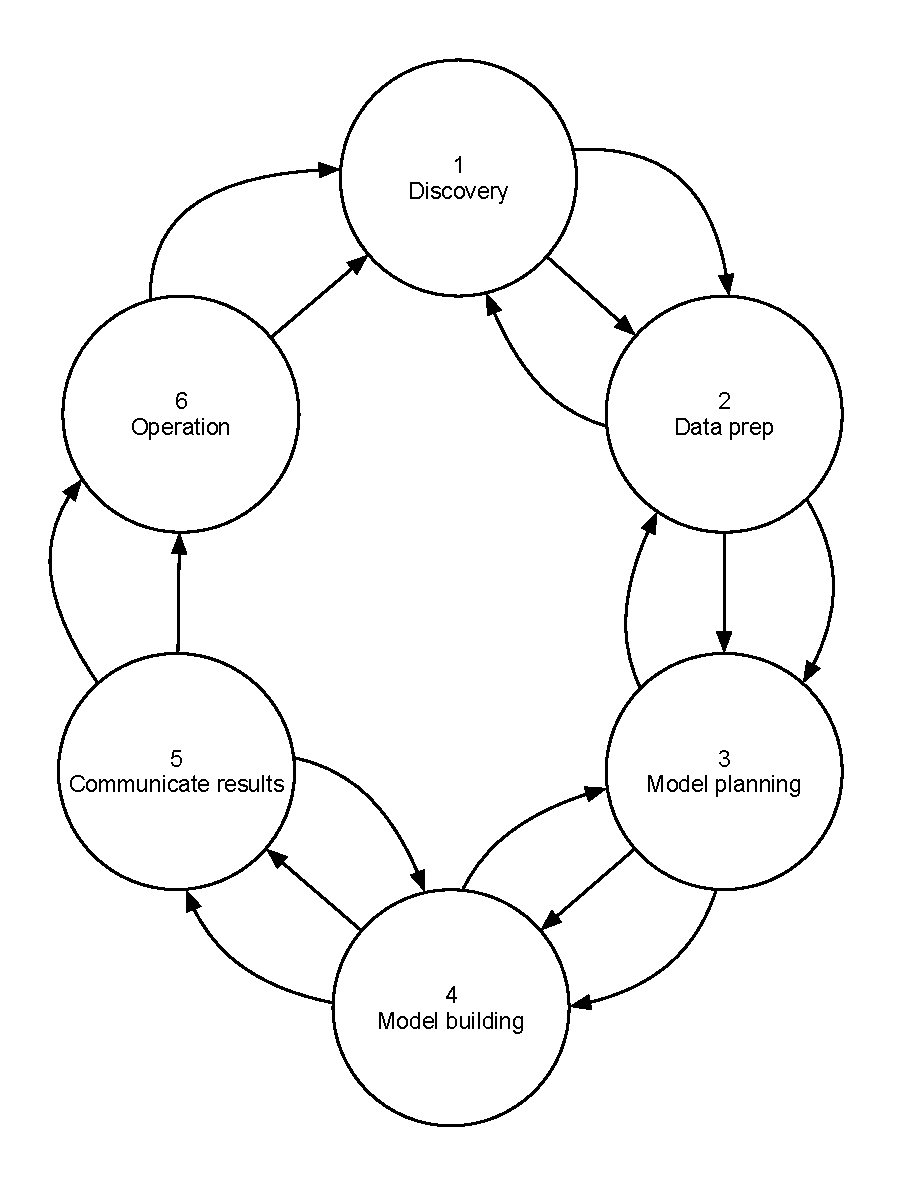
\includegraphics[width=8cm]{./figures/datalifecycle.eps}
\caption{Data Analytics lifecycle \protect\cite{STOREY201750}}
\label{fig:lifecycle}
\end{figure}

\section{Model Overview}

In recent years, research and development have been focused on creating a streamlined, widely acceptable data analytics lifecycle.

The goal of the data analytics lifecycle was to have a structure in place that could aid developers and other researchers. Teams usually learn new things throughout their projects and often need to go back to the previous phase to refine their work based on new insights and information they have uncovered \cite{dietrich2015data}. 
Each component of the data analytics lifecycle will briefly be discussed below:

\begin{enumerate}
    \item Discovery – in this phase, discovering and gathering data is undertaken. It is essential to frame the data needs best and to obtain the correct data according to the requirements.
    \item Data preparation – the data must be correctly formatted to be used in a later phase.
    \item Model planning – this phase entails looking at various methods, techniques, and workflows that need to be employed to learn about the underlying relationships between the variables.
    \item Model building – also known as analyze data, this phase focuses on analysing the data and determining whether the existing tools will suffice to get to the end goal.
    \item Communicate results – in this phase, various visualisation techniques will be considered and a summary will be developed to convey to the stakeholders.
    \item Operationalise – this is also commonly known as making decisions. This phase focuses on delivering reports, code, and other technical documents.
\end{enumerate}

\begin{table}[htbp]
\centering
\begin{tabular}{|l|l|l|}
\hline
\textbf{Known terminology} & \textbf{Study terms} & \textbf{Domain of techniques} \\ \hline
Discovery & Past papers & Dataset\\ \hline
Data prep & Preprocessing & Machine learning - Chapter \ref{ssec:prep}\\ \hline
Model planning & Learning & ML + IR - Chapter \ref{chap: Chapter 3} \\ \hline
Model building & Human intervention & Prototype - Chapter \ref{ssec:prot} \\ \hline
Communicate results & Represent in data frame & Discussion - Chapter \ref{chap: Chapter 7}\\ \hline
Operation & Enable decision makers & Evaluation - Chapter \ref{ssec:eval} \\ \hline
\end{tabular}
\caption{Mapping between Terminologies Used in the Study}
\label{tab:mapping}
\end{table}

\begin{figure}[htbp]
\centering
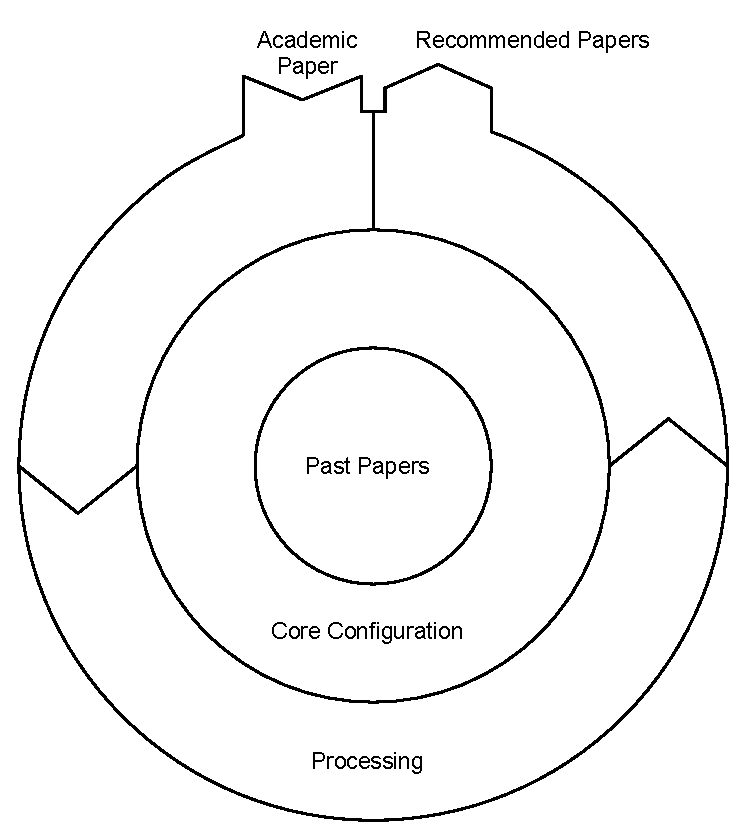
\includegraphics[width=8cm]{./figures/overview3.eps}
\caption{The Model Overview}
\label{fig:Modeloverview}
\end{figure}

With the above being said, the researcher felt the need to provide a mapping between the terminology used in the research domain and this study. As seen in Table \ref{tab:mapping}, it should be known that when the researcher uses terminology like past papers, pre-processing, and learning they hold the exact content of the corresponding terms used in research. The column on the right in Table \ref{tab:mapping} can be translated to be the domain and/ or section in this study which addressed each phase of this model.

This section of the chapter covers the model overview, as seen in Figure \ref{fig:Modeloverview}. The model is categorised into three components: (1) past papers, (2) learning, and (3) processing.

Past papers can be identified as the core of the model. It is made up of past or historical papers. This will then flow into the learning component, which is a fundamental stepping stone in defining what needs to be done. In the processing component, the model looks at the defining functions in learning and further refines them. The learning and the processing component will be discussed further in this chapter.

\section{Learning}

The learning component is created by analysing past papers closely. The goal was to understand better the characteristics which made up the learning component. The conceptual model is constructed in such a way that it is not only information security domain-specific. This being said, the characteristics of the learning component were identified and guided by literature. The characteristics of the learning component are:

\begin{enumerate}
    \item Populating the stopword list
    \item Stemming
    \item Topics of the model
    \item Measuring the similarities
\end{enumerate}

\begin{figure}[htbp]
\centering
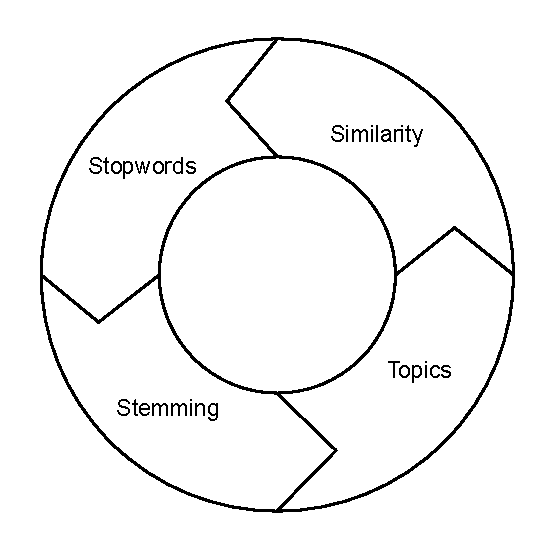
\includegraphics[width=8cm]{./figures/learning.eps}
\caption{Learning Component}
\label{fig:core}
\end{figure}

The flow of the learning component is using the stopword list, then stemming those words. Stemming leads into topics that will be generated, and the similarity of these topics will be measured. As seen in Figure \ref{fig:core}, the flow of the learning component  leads one character into another. The reason for this is that the learning component is a continuous process. Each of these characteristics is described in the following sections.

\subsection{Populating stopword list}

The stopword list was primarily made up of NLTK’s stopword list. The goal of this choice was to employ a stopword list with a comprehensive list of words. NTLK is one of the most widely used NLP libraries. Furthermore, after close consideration, additional words were included in the stopword list as time passed. These words were primarily domain-specific such as: (1) information, (2) technology, and (3) security.

The goal of the inclusion was to retrieve second- or third-tier topics from the text. The textual outputs of each component of the learning component were analysed, and words that did not bring any value or primarily domain-specific words were omitted.

The process of including some words and excluding others was a manual and iterative process. The resulting words were best suitable for the information security domain and were used as the stopword list.

\subsection{Why Stemming?} \label{ssec:stemming}

Stemming was employed for the sheer simplicity and thorough work it has done. To recap, stemming is removing the suffix of the word to return it to its root form. The Porter stemmer is appropriate to IR research work involving stemming where the experiments need to be repeatable exactly. This being said, after consulting the dataset, it was identified that the domain in which this research position found itself did not need to have a custom-made stemming solution.

After close consideration, the researcher, along with evidence, used Porter stemmer from the NLTK library.

\subsection{Topics of the model}

The information technology domain is such a rich field with regard to topics and sub-topics. It needed to be scoped down to provide better topics for the algorithm to use. For example, information, technology and security would be excluded. As seen in Section \ref{fig:core}, all of the components fed into one another. In this case, specific topic names were appended in the stopword list. 

The result of the methodology mentioned above was smaller topics. These were second- and third-tier topics, such as hacking and man-in-the-middle attacks, respectively. A few of the lower-tier topics fused to make up the second-tier topics. This also holds for second-tier- and first-tier topics.

\subsection{Measuring the similarities}
The vast number of topics made it challenging to group similarities of papers. The topics were too dense from the perspective of dimensionality. For the scope of this research, similarity algorithms reduced dimensionality. In addition to the dimension reduction, the unsupervised learning approach made it viable to use an algorithm to cluster similar topics. This would have a direct impact on measuring the similarities in the academic papers.

\section{Processing}

In this section, the next phase of the conceptual model will be discussed. The academic paper processing phase is executed when a new and unseen academic paper is submitted. Just like the learning component, this phase also has four components. It is merely an extension of the components found in the learning component.

In the first step, the fundamental stepping stone was actioned, the removal of stopwords. The new document had its stopwords removed to simplify and get the text ready for further analysis. Step two includes taking the text that was cleaned and stemming it. This removed the suffix and returned the words to their root form. The goal of Step three was to get the related topics in the text. The last step, Step 4, focused on using the topic output and determining the similarities of the topics. These four components are best described in Figure \ref{fig:processing}, and a brief description of each component is given in the following sub-sections.

\begin{figure}[htbp]
\centering
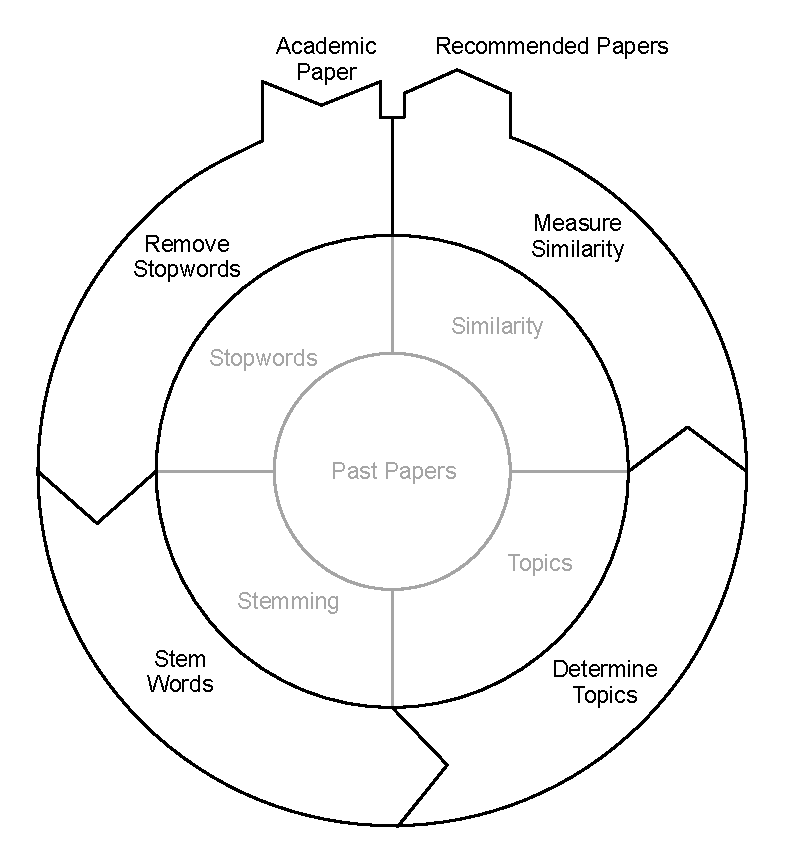
\includegraphics[width=8cm]{./figures/processing1.eps}
\caption{Processing phase of the model}
\label{fig:processing}
\end{figure}

\subsection{Removing the stopwords}

The stopwords are removed from the collection of documents. The goal was to remove the words that do not bring any meaning to the sentences. These are terms such as ’specified’ , ’specify’, ’specifying’. The stopword list also included words such as ’information’, ’security’ and ’technology’.

\subsection{Stemming of the words}

After the stopwords were removed, the tokenised dataset was then stemmed. For example, the words mentioned above: ’specified’ , ’specify’, ’specifying’ can be stemmed and will look like the following: ’specif’, ’specif’, ’specif’. As explained in the learning component section of this chapter, stemming is removing the suffix of the word to return the term to its root form. The stemmed words are then used to determine topics.

\subsection{Determining the topics} \label{ssec:topic}

This component comprises determining the topics of the dataset. This is done after the stopwords were removed and after the text was stemmed.
A topic modeling technique was then applied to the dataset after it was transformed. The soft clustered topics looked something like this: ’0.040*”data” + 0.033*”file” + 0.024*”encrypt” + 0.021*”cloud”. A similarity ratio of the terms was calculated, and the most similar terms were clustered together, forming topics.

\subsection{Measuring the similarities}

At this point of the conceptual model, the stemmed words that did not contain any stopwords were pushed through the topic modeling technique. The product of the previous three components was a collection of topics that represented the dataset. The collection of topics of the dataset and the topics of the test set were measured in terms of similarity. The lower the score, the more similar the two papers were with one another.

\subsection{Processing phase summary}

In this section, we discussed the academic paper processing phase. This phase was executed when a new document was submitted. The dataset already removes the stopwords, stemmed, and determined the topics. Once a new document was submitted, it went through the same process. The only difference there was that the similarity of the two datasets were then measured. The topics with the lowest score were most similar.

\section{Summary}

The conceptual model presented in this chapter is a template for finding similar academic papers. The use case for this research was focused on information security academic papers. However, it can be used to find any academic papers across disciplines. The conceptual model was built on a collection of academic papers or datasets. Various learning components were identified while surveying the field. The learning components were broken down into four distinct components: (1) stopword, (2) stemming, (3) topics, and (4) similarity.

After the learning component was built through experimentation, it was ready and waiting for new academic papers to do the testing. The academic paper processing phase could then begin. Just like the learning components, the academic paper processing phase also has four components.

First, the dataset was cleaned of all the stopwords. Special consideration was made for the first-tier topics like ’information’ and ’security’, and those were also included in the stopword list.

Second, once the stopwords were removed, next would be to stem the remaining data. Stemming commonly includes omitting the suffix of a word. This was done to return the word to its root form.

Third, topics were determined by using a topic modeling technique. The technique helped soft cluster all of the similar terms together, which formed topics. These topics consisted of the ’training set’ corpora. Once a ’test set’ document appeared, it was run through the same components.

Once we had the ’training set’ and ’test set’ ready, the last component measured the similarity between the two sets. The new, unseen ’test set’ document was then hard clustered to the most similar set of topics. In the next chapter, the prototype development will be discussed.
